\chapter{Introduction}
\label{c:introduction}

In human-computer interaction (HCI) research, the study of the relation between users and systems is of interest. Within the context of games research in particular, the relation between player and game is an important topic. Such relation comprehends concepts as engagement and immersion \parencite{boyle2012engagement} and the investigation of the elements that influence those concepts. Researchers and practitioners benefit from tools to perform the aforementioned investigations, such as the ones illustrated in the following hypothetical scenarios.

\textbf{Scenario 1:} a games researcher wants to investigate the stress level of a user during a training session with a serious game. The researcher points an ordinary camera at the user's face and asks him/her to play a few games for 15 minutes for calibration purposes. After that, the researcher records a video of the user's face while he/she plays the serious game to be investigated. The user experience is not disturbed by inconvenient sensors attached to his/her body, nor is the user constantly interrupted during the game play to answer questionnaires. After the user finishes playing, a software shows a report informing the researcher about the stress levels throughout the session. On another occasion, the researcher asks the same user to play a different serious game being investigated. This time the researcher skips the calibration phase because the profile of that user is already known (no re-calibration phase is needed). Again the researcher points a camera at the user's face, films the gaming session and at the end a software shows a report regarding stress levels.

\textbf{Scenario 2:} a small game developer company wants to check if a new title to be released is well balanced, i.e. it is not too difficult nor too easy to play. The small company has several hours of video recordings of users play-testing the game, however they have no budget nor time to manually inspect the material to find useful information. A representative of the company then invites the users involved in the play-testing sessions to visit the company again. A new video of each player is recored while he/she plays a few calibration games for about 15 minutes. After that, the company representative feeds a computer software with the newly created user videos and the already existing videos with hours of gameplay. In minutes, all material is analyzed and a software indicates the points in time where the stress level of users was higher than their usual behavior. The company then inspects the problems and adjusts the games accordingly, increasing its chances of success.

The mentioned scenarios illustrate the investigation work-flow of researchers and practitioners when using a novel process that is the research aim of this thesis. Currently researchers perform such investigations relying on obtrusive and cumbersome methods that are able to capture the user's emotional state. The most commonly used techniques to obtain data regarding emotional states of players in a game are self-reports (questionnaires) and physiological measurements \parencite{mekler2014systematic}. Questionnaires are practical and ease to use tools, however they require a shift in attention, hence breaking or affecting the level of engagement/immersion of the user. Physiological signals, on the other hand, have been used to obtain information from users without causing interruptions \parencite{bousefsaf2013remote,yun2009game,rani2006empirical,tijs2008dynamic}. Sensors, despite avoiding interruptions, are usually perceived as uncomfortable and intrusive, since they require the proper setup in the person's body. Additionally sensors might restrict player's motion abilities, e.g. a sensor attached to a finger prevents the use of that finger. Sensors also increase user's awareness of being monitored \parencite{yamakoshi2007preliminary,yamaguchi2006evaluation,healey2005detecting}, which disturbs the results of an investigation.

%Questionnaires, however, require the user to stop the game activity in order to share his/her current state. The frequency that such questionnaires are issued is also a concern. If performed too often, more information might be collected, but the data might contain noise caused by the frequent interruptions, e.g. player is more stressed/bored by the questionnaire interruptions than by the game itself. If performed too sparse, not enough information will be gathered from the player.

Despite the mentioned problems, sensors continue to be used because there is a significant amount of information that can be read from the human body, such as heart rate (HR), respiratory rate (RR), facial expressions, among others. Such information in the human body can be seen as input signals for emotion estimation. A number of studies \parencite{kukolja2014comparative} suggest that the analysis of a combination of different input signals, known as multimodal or multifactorial analysis, is more likely to produce accurate results when mapping emotional states. Physiological signals, e.g. HR, are considered reliable sources since they are hard to fake (because of their link to the central nervous system), differently from facial expressions \parencite{Landowska}, for instance. When combined in the same analysis, however, those signals can complement each other and provide more information about emotional states. The process of mapping such signals to an emotional state, however, is a significant task. It involves testing/defining what are the possible emotional states a person can experience \parencite{mandryk2006continuous}, as well as comparing which signals are better predictors of such states \parencite{jerritta2011physiological}. A common approach to perform the mapping between input signals and emotional states is the use of machine learning models.

The use of a machine learning model commonly starts by exposing a group of users to some emotion elicitation material, e.g. images and videos with known emotional labels as stress and boredom. Signals from those users, e.g. HR and facial expressions, are measured during the interaction and used to train the machine learning model according to the labeled elicitation material. Ideally the trained model can be generalized and used to detect the emotional state of different users based on the analysis of their signals. This approach, however, fails to learn individual nuances since it assumes all users behave similarly. In practice, this approach is limited to detecting the average behavior of the training group. The great variability between individuals regarding physiological signals and emotional states does influence the process. Studies have shown that the correlation between facial analysis and emotional states of the training population significantly differs from the expected correlation described in the literature for other populations \parencite{grafsgaard2013automatically}. Additionally there are indications that a machine learning model presents higher prediction rates for users with the highest self-reported emotional levels during the training phase, as well as the lowest prediction rates for participants with the lowest self-reported emotional levels during the training phase \parencite{mcduffcogcam}. It emphasizes the individualities of each user and the need of a user-tailored approach that preserves such characteristics.

Investigations towards a user-tailored approach can be found in the literature. It has been proven that a model created from a group of users is less effective at detecting emotions than a model created from a single person which is used to analyze that same person in the future \parencite{bailenson2008real}. This user-tailored approach is more likely to learn individual characteristics, not the average features of the training population. Additionally some works show a migration from physical, obtrusive approaches for signal acquisition of users in favor of remote-based approaches. Advances in areas such as computer vision allow the remote acquisition of input signals, including HR information, based on the analysis of videos of users. Remote detection of HR, for instance, proved a promising approach to infer boredom/stress levels \parencite{kukolja2014comparative} or cognitive stress \parencite{mcduff2014remote} of a person. Such a remote and non-obtrusive approach, combined with a user-tailored machine learning model, allows the development of new tools for emotion detection.

This thesis presents an approach built on the previously mentioned studies applied to the context of games. \textit{The main contribution is the detection of emotional states of users during gaming sessions using remote acquisition of signals via computer vision, a user-tailored model and emotion elicitation based on a novel game-based calibration phase. The approach is automated and implemented as a software without the need of specialized equipment, e.g. sensors, only a regular video camera}.

%Research in different areas, such as affective computing and computer vision, aim to improve the workflow of emotion investigation with non-obtrusive approaches involving the aforementioned signals. By using computer vision and a video stream captured by a camera, one can obtain different information from a subject, such as facial expressions and physiological signals, without the use of physical sensors.

The following sections present how the proposed approach can be achieved, showing the problem specification, the research aim and its contributions.

\section{Problem specification}
\label{sec:problem-specification}

As previously described, questionnaires and physiological measurements using intrusive sensors are the most common approach used to obtain data for emotion estimation. Both approaches interfere with the natural behavior of users, which affects any research procedure. Improvements to such approaches have been proposed in the literature, including the use of computer vision for remote extraction of user signals and a user-tailored machine learning model to map those signals into emotional states. The material used for emotion elicitation is also an important component of the process to accurately capture the singularities of each user.

One of the problems with previous work is directly connected to the emotion elicitation material used in the process. In the majority of the existing studies, subjects had limited interaction with the content being presented: they performed tasks mentally (e.g. counting), watched videos/images or performed gamified cognitive tests for a short period of time. Those are artificial situations that are unlikely to happen in a context involving games. The models trained from those emotion elicitation sources are less likely to cover the range of emotional activity featured by users during gaming sessions, especially those with a challenging game lasting for several minutes. There is a lack of investigation regarding the use of games as emotion elicitation sources, which is of interest to the games research community. The process of detecting emotions of users while they play games is more likely to succeed with a model trained from game-based emotion elicitation materials instead of images and videos. With game-based emotion stimuli, users take an active role in the process, making decision and directly interacting with the content. It results in more genuine emotional manifestations. When images, videos or gamified tests are employed, users take a passive role with limited possibilities for interaction or emotional involvement, resulting in less significant emotional manifestations.

Regarding the initiatives based on computer vision and emotion estimation, remote detection of HR, for instance, proved a promising approach to infer boredom/stress levels \parencite{kukolja2014comparative} or cognitive stress \parencite{mcduff2014remote} of a person. The application of such techniques, however, has not been proposed in a context involving games and natural behavior of users. Experiments regarding the use of computer vision and signal extraction were performed under extremely controlled situations with few game-related stimuli. A significant limitation of such approaches was that subjects were asked to remain still during the experiment. This is an uncommon user behavior during the interaction with emotional stimulation that hinders the real efficiency of such remote detection techniques. In particular, when game-based emotion elicitation is used, users are likely to behave in a more natural way, e.g. featuring facial expressions and moving the body \parencite{bevilacqua2016variations}, which directly affect the remote measurements of physiological signals. The use of such computer vision techniques within the context of games and natural behavior must have its reliability confirmed. Additionally the techniques must be adapted to overcome the challenges associated with its usage in the context where users behave naturally while playing games instead of being oriented to remain still.

Finally previous works focus on predictive models based on a collective perspective. As a consequence, a model is usually trained from data of several users, which in practice describes the average behavior of the group, excluding key individualities of each user. Such individualities are the main characteristics that define a person, since people are different in many aspects, including expectations regarding culture and personal belief \parencite{goldberg1993structure}. It has been proven that a user-tailored approach is more likely to produce better emotional estimations \parencite{bailenson2008real}, however no previous work has focused on game-based emotion elicitation combined with a user-tailored model. It is reasonable to believe that those individual characteristics might be better observed with a more personalized and complex emotion elicitation materials such as games. Furthermore a user-tailored approach is likely to preserve and better account for individual characteristics in a method for emotion detection, as opposed to a group model to detect emotions. Additionally models created from a group are highly affected by ethnical and gender bias, since it is significantly difficult to obtain data from a group that accurately represents the world population. Such limitation is inexistent in a user-tailored model, since the approach is, by design, based on data of a single person that already is a perfect representation of him/herself.

In summary, previous works focus on models trained from data of a population instead of a user-tailored approach. It dilutes the peculiarities of each user and tends to predict the average behavior of a group. When a model is used, it is trained with emotion elicitation materials based on images \parencite{giannakakis2017stress,anttonen2005emotions}, videos \parencite{bailenson2008real,grundlehner2009design} and gamified cognitive tests \parencite{mcduff2014remote,mcduffcogcam}. The use of games as emotion elicitation sources is not fully explored. The acquisition of user signals, e.g. HR and facial expression, is performed remotely via computer vision, however its applicability in a context involving games and natural behavior lacks further investigation. In that light, there is a lack of initiatives focusing on \textit{non-obtrusive}, \textit{user-tailored} emotion detection models, in particular regarding \textit{stress} and \textit{boredom}, within the context of \textit{games research} that are based on emotion data generated from \textit{game stimuli}. This thesis presents a research that aims to fill that gap, providing the games research community with a process to remotely detect the emotional state of users in a non-obtrusive way, based on a model trained from a novel game-based calibration phase, which directly relates to the context of games research.

\section{Research aim}
\label{sec:research-aim}

The aim of this research is to produce an emotion detection process that relies on computer vision to remotely acquire psychophysiological signals from a person to detect his/her emotional state regarding stress and boredom. The emotion detection is based on data obtained in a game-based calibration phase.

The overarching research question is the following:

\begin{fquote}
How can the emotional state of players during the interaction with games be remotely detected on a user-tailored basis with the utilization of an ordinary camera and games as emotion elicitation sources for calibration?
\end{fquote}

The following research objectives (O) have being identified to support the overall aim of this project:

\textbf{O1}: identification of the main concepts, theories and signals associated with the psychophysiological profile of users and their emotions within the field of HCI, particularly regarding games research. The outcome of this objective is a definition of stress and boredom within the context of this research, as well as the identification of which psychophysiological signals are commonly applied to emotion detection.

\textbf{O2}: identification of existing computer vision techniques that can be employed to remotely extract the identified psychophysiological signals of users via analysis of videos. The investigation includes the analysis of how existing techniques are being applied to emotion detection. The set of signals to be remotely extracted is based on the results of objective \textbf{O1}.

\textbf{O3}: investigation of the feasibility, accuracy and challenges of applying the identified computer vision techniques regarding the extraction of the signals within the context of computer games. This objective also comprehends the analysis of the behavior of players during gaming sessions and how it affects the technique.

\textbf{O4}: investigation and validation of the concept of a game-based calibration phase as an emotional elicitation source able to provide data to fit a user-tailored predictive model. The result of this objective is to design and validate a set of calibration games that can trigger the emotional responses required for the analysis of the remotely obtained signals and detection of boredom and stress levels by the model.

\textbf{O5}: proposal of a user-tailored, multifactorial model that uses the identified physiological and non-physiological signals, the computer vision technique and the calibration data to detect the current stress/boredom levels of a person while he/she plays any video game.

\textbf{O6}: experimental validation of the proposed emotion detection process with an experiment involving a commercial off-the-shelf game.

%The proposed method will be based on the analysis of the variation of signals of a person according to a reference (calibration data). This approach is significantly different from the already existing methods, which focus on training a model to detect pre-defined states (e.g. stress, boredom, rest) based on the current value of the acquired signals. The foundation of the approach proposed in this research is the use of variations, which by nature account for differences between the current state and any other known state (the calibration profile, for instance). This configuration allows the method to be expanded or further investigated to produce a scale regarding the measurement of stress and boredom. Different from a direct mapping of signals to a state, a scaled measurement might inform the researcher of how much stress or boredom the player is experiencing, as opposed to just informing he/she is stressed or bored. This might be possible to be achieved with a machine learning model, for instance, but it will require a complex training setup. which will inevitably result in frequent interruptions of the player for collecting self-reported stress/boredom levels. This will disturb immersion/engagement with the game, probably resulting in noise in the mapping.

%A researcher is be able to increase the internal validity of his/her workflow by ensuring the player keeps the focus on the game without interruptions and by minimizing the side effects (and inconveniences) of physical monitoring. This research can also be deployed as a solution for game developer studios to automatically analyze hours of recorded gameplay and highlight the moments when boredom/stress levels changed significantly. As a complement the solution is based on a single, ordinary camera and a software implementation, which eliminates the use of complex setups of physical sensors. It eases the investigation process and reduces costs.


\section{Knowledge contributions}
\label{sec:contributions}

The result of this research adds to the body of knowledge of HCI and games research. Information regarding concepts, models and theories involving games, emotions and computer vision were identified, evaluated and orchestrated to work in combination. The main knowledge contribution of this research is a novel process for emotion detection that is remote, non-intrusive and constructed from a game-based, multifactorial, user-tailored calibration phase. The process is able to detect stress/boredom levels of users during the interaction with games.

The proposed emotion detection process \textit{per se} is the main contribution, however it is composed of different parts that possess individual contributions on their own. Below is a list with all those individual contributions and their relation to the research objects mentioned in section \ref{sec:research-aim}:

\begin{itemize}
  \item The concept of calibration games, which are games with specific characteristics used as emotional elicitation sources to identify an emotional profile of users (\textbf{O1} and \textbf{O4}).
  \item Game-based calibration process that uses calibration games to train a machine learning model for emotion detection regarding stress and boredom (\textbf{O4} and \textbf{O5}).
  \item Identification and adaptation of computer vision techniques suitable to remotely extract user signals in a context involving games and natural behavior (\textbf{O2} and \textbf{O3}).
  \item A multifactorial, user-tailored machine learning model that maps a set of remotely acquired user signals, e.g. HR and facial actions, into emotional states related to stress and boredom (\textbf{O1}, \textbf{O4} and \textbf{O5}).
  \item Validation of the proposed emotion detection process in an experimental setup (\textbf{O6}).
\end{itemize}

The purely remote-based approach proposed by this research enhances the available methods for the investigation of emotional states of stress and boredom. The approach, which is based on novel a user-tailored, game-based calibration phase, maps a set of variations of signals into two specific emotional states, i.e. stress and boredom. This information can be used by other researchers to identify important moments during the interaction of players with games, such as when the recognized pattern is closer to stress. In game design research, for instance, that instrumentation can be used as another way of obtaining information from a user during a game session. The use of questionnaires, which shift the player's focus away from the game, can be enhanced and/or replaced by the use of the proposed method, making the process less obtrusive. By remotely reading information regarding stress and boredom, a researcher can use such information to better understand concepts as engagement, frustration, immersion and flow in games, for instance. Additionally it can be used in any activity that relies on stress/boredom as an important measurement, such as usability tests in software and games, for instance. Another contribution is a better understanding of how the selected signals are related to stress/boredom. Other researchers might use that information in contexts outside the area of games research, such as the measurement of costumers satisfaction or interest in stores.

The general structure of the proposed process is illustrated in Figure \ref{fig:research-aim-general}. The process contains two main phases: a calibration and an emotion estimation phase. In the calibration phase, the user plays a set of carefully designed games, named calibration games, that act as emotion elicitation sources. During this phase, the user signals elicited from the interaction with the games, e.g. HR and facial expressions, are remotely acquired and used to train a user-tailored model. This model is the foundation to detect stress and boredom levels of that particular user in any other game. In the emotion estimation phase, the user interacts with any ordinary game, e.g. serious game, while his/her signals are remotely acquired and fed into the previously trained user-tailored model. The model outputs the current levels of stress and boredom for that user in that game.

\begin{figure}[h!]
    \centering
    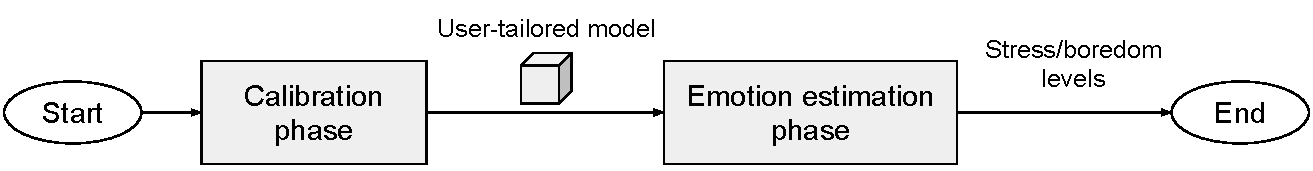
\includegraphics[width=\textwidth]{Content/figures/research-aim-general}
    \caption{General structure of the proposed method for remote detection of stress and boredom levels of players during the interaction with games.}
    \label{fig:research-aim-general}
\end{figure}

The process is based on a non-contact, multifactorial analysis of user signals obtained from a video stream via computer vision. The principal of the emotion detection phase is based on a user-tailored machine learning model, which is trained with information obtained from the user while he/she played a set of games in the calibration phase. The user-tailored machine learning model is trained according to the process presented in Figure \ref{fig:user-tailored-calibration}. Each user plays a set of calibration games while being recorded by a camera. Computer vision is used to process the video feed and remotely extract signals from the user, such as HR and facial actions. Those signals are used as input to train the machine learning model for that particular user (user-tailored model).

\begin{figure}[h]
    \centering
    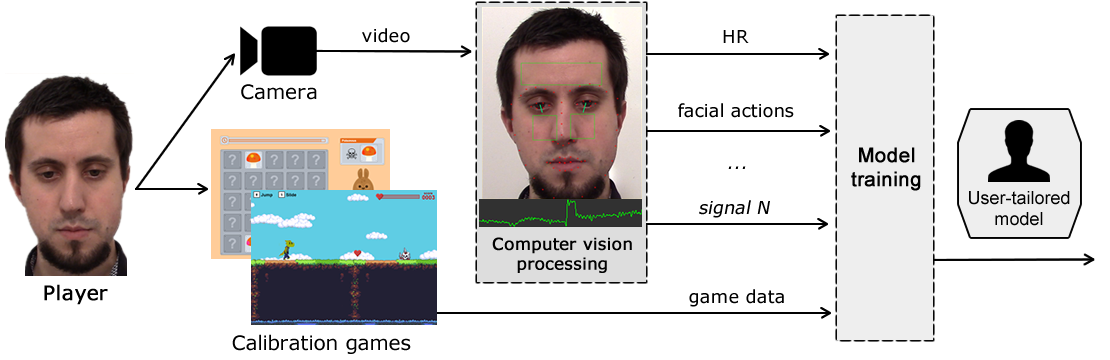
\includegraphics[width=\textwidth]{Content/figures/user-tailored-calibration}
    \caption{Calibration phase composed of emotion elicitation games (calibration games) and remote acquisition of signals from the user. The result of this phase is a user-tailored model used to detect emotions.}
    \label{fig:user-tailored-calibration}
\end{figure}

The games used in the calibration phase act as emotion elicitation sources. Each of those games are casual-themed and carefully designed to trigger two distinct emotions, i.e. boredom and stress, featuring a progressive transition between them as illustrated by Figure \ref{fig:calibration-game-linear}. At the beginning of the game, the difficulty level (green line) is low and the user is required to perform few or no actions. The games are designed in a way that the user is not able to increase the pace of the gameplay nor make it faster based on personal skills. As a consequence the user is forced to play a low-paced gameplay, which leads to an emotional state of boredom (blue curve). As time progresses, the pace of the gameplay and its difficulty level increase linearly. The increase happens at fixed time intervals, e.g. every 60 seconds. At some point in time, which is different for each user depending on gaming skills and personal preferences, the pace of the gameplay and the difficulty level will be overwhelming, leading the user to an emotional state of stress (red curve). As the difficulty level continues to increase, the stress level of the user will also increase. Finally the difficulty level will increase until the point where the user is unable to cope with the game, which will lead to consecutive mistakes in the game that will eventually terminate it, e.g. heath bar of the main character reaches zero.

\begin{figure}[h!]
    \centering
    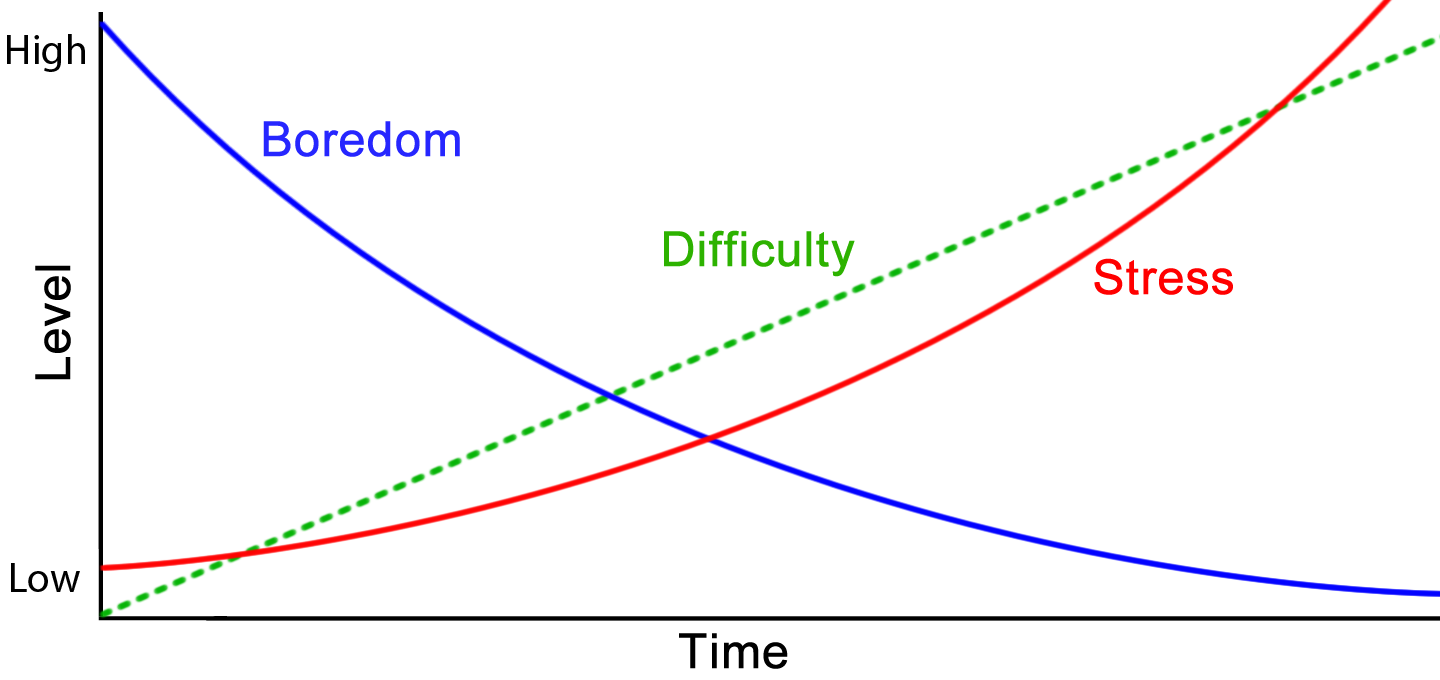
\includegraphics[width=0.7\textwidth]{Content/figures/calibration-game-linear}
    \caption{Progression of the level of difficulty of a calibration game over time along with the corresponding variations of the emotional states of stress and boredom experienced by the user.}
    \label{fig:calibration-game-linear}
\end{figure}

The mentioned calibration games are designed to trigger specific emotions and vary them over time, so the remotely collected information from the user during the calibration phase contains a detailed variation profile of the person being analyzed, including changes of each signal and the theoretically known emotional state of the user at that moment. If a person has a better response to a certain physiological signal instead of another, e.g. HR over facial expressions, then the variation of that signal accounts more weight in the training of the model. Since the training process is completely based on the signals of a single user, nuances and individual behavior are likely to be registered and learned. The calibration phase needs to be performed once per person.

After the calibration phase, the person can play any other ordinary game and be monitored in an emotion estimation phase, as illustrated by Figure \ref{fig:user-tailored-use}. As the user plays the game, signals are remotely acquired via computer vision. Those signals are used as input to the trained user-tailored model of that particular person, which produces as a result an estimation of the emotional state regarding stress and boredom for that person in that game. The process relies on the same remotely acquired signals with the addition of the predictions of the model according to the training performed during the calibration phase.

\begin{figure}[h]
    \centering
    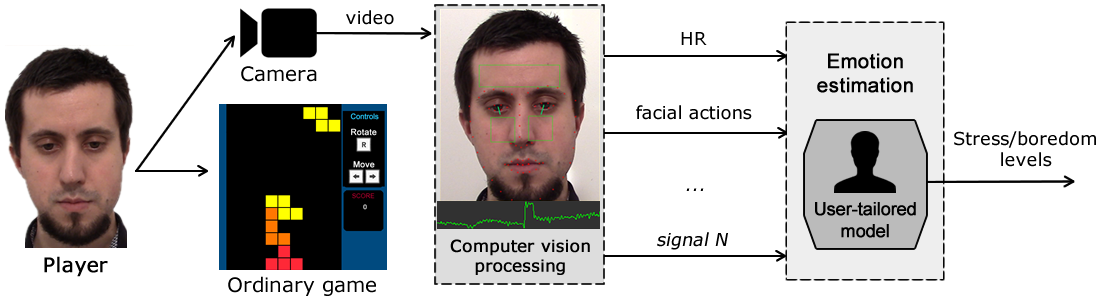
\includegraphics[width=\textwidth]{Content/figures/user-tailored-use}
    \caption{Emotion estimation phase. Remotely acquired signals from the player are fed into a user-tailored model that outputs the stress/boredom levels of the player during the interaction with an ordinary game.}
    \label{fig:user-tailored-use}
\end{figure}

Given that the user has a trained user-tailored model, the emotion estimation phase can be performed for any game as many times as desired. The model uses the remotely obtained signals from the user in conjunction with the calibration data to detect the player's changes regarding stress and boredom levels in any other game.

%According to previous research, the use of games as a emotional triggering mechanism is a feasible approach. Additionally an user-tailored model is a more efficient approach than a group-tailored model for the detection of emotional changes in users.
%\section{Thesis overview and structure}

\section{Thesis overview and structure}

This thesis is divided in parts whose chapters present and explain in details the scientific methodology, the theoretical background and the studies conducted to achieve the research aim described in Section \ref{sec:research-aim}. Overall the solution to remotely detect user emotions proposed by this thesis relies on three main elements: \textbf{emotion elicitation}, i.e. calibration games, \textbf{acquisition of users signals}, i.e. computer vision techniques, and \textbf{emotion estimation}, i.e. user-tailored machine learning model. Those three elements are significantly intertwined and they directly affect each other. In summary, when users interact with game-based emotion elicitation material, they tend to move, laugh and occlude the face, which adds noise to (or impede) the estimations performed by the computer vision techniques. It then affects or even prevents the creation of an emotion detection model, which requires the games to be re-worked or adapted to ensure they continue to serve as emotion elicitation material, consequentially leading to a chain reaction that cycles over the previously mentioned elements again.

According to the literature review conducted for this research, the use of those three main elements combined has never been tried before. As a result, it was not possible to determine beforehand if they could actually work in combination to detect user emotions remotely. A set of iterations would be required to test, evaluate and learn about those elements working together. On that account, Design Science, an iterative problem solving research method, was deemed the best approach to conduct the investigation, as explained in Chapter \ref{ch:methodology} (on page \pageref{ch:methodology}). Using such research method, the literature is consulted and a tentative solution is proposed and evaluated. Results of such evaluation provide new insights about the problem, which are then interpreted against the literature, leading to a new tentative solution. The cycle is repeated until a solid contribution is formed. For the research conducted in this thesis, the literature review made it clear that a more fruitful way of detecting emotions would be to interpret them as a manifestation of psychophysiological signals, e.g. HR and facial activity. It steers the research towards human physiology instead of psychology, whose interpretation is likely less subjective and more quantitative oriented. The literature review also focused on identifying which psychophysiological signals have been used in previous work focused on emotion detection, along with identification of computer vision techniques that can remotely extract those signals. After selecting the set of signals and computer vision techniques to be used in this research, six iteration of the design science cycle were performed based on two experiments. Experiment 1, detailed in Chapter \ref{ch:experiment1} (on page \pageref{ch:experiment1}), aimed to evaluate the feasibility of using the previously mentioned three main elements of this research in conjunction. It was mainly designed to test if the concept of calibration games, a novel aspect of the this thesis, would cause an emotional reaction on the subjects that could be remotely detected out of psycophysiological signals. Data gathered in experiment 1 was analyzed in five studies, i.e. Study 1 to 5, which can be seen as five iterations in the design science cycle.

\textbf{Study 1:} detailed in Section \ref{sec:experiment1-study1} (on page \pageref{sec:experiment1-study1}) was an exploratory evaluation of facial activity and perceived boredom and stress levels. The evaluation is connected to previous works and emotion/game theories presented in Chapters \ref{ch:literature-games} and \ref{ch:literature-face} (on pages \pageref{ch:literature-games} and \pageref{ch:literature-face}, respectively). Analysis of subject's self-reported emotional states statistically confirmed that they perceived the games as being boring at the beginning and stressful at the end. It supported the idea that calibration games, a corner stone in this thesis, could be used as emotion elicitation material. Additionally manual and empirical analysis of the video recordings indicated that subjects presented more facial actions during stressful periods of the games compared to boring periods. Finally there was indications that subjects featured a neutral face most of the time, which implies that it is not trivial to estimate emotions purely based on facial analysis without a context.

\textbf{Study 2:} detailed in Section \ref{sec:experiment1-study2} (on page \pageref{sec:experiment1-study2}) evaluated if calibration games could produce variations in physiological signals, namely HR, as described by the theories and previous work presented in Chapter \ref{ch:literature-physiological} (on page \pageref{ch:literature-physiological}). Analysis of the HR collected with a physical sensor, i.e. watch, during the experiment statistically confirmed that subject's HR was different during stressful and boring periods of the game. This information confirmed that calibration games could be used as emotion elicitation material, effectively inducing variations in physiological signals on subjects exposed to them, which could be used to detect emotions.

\textbf{Study 3:} detailed in Section \ref{sec:experiment1-study3} (on page \pageref{sec:experiment1-study3}) evaluated the feasibility of remotely detecting the variations of HR that were confirmed in Study 2. Remote photoplethysmography (rPPG), as described by the theories and works presented in Chapter \ref{ch:literature-rppg} (on page \pageref{ch:literature-rppg}), was used as the technique to remotely estimate HR information from videos of subjects interacting with games. Estimations of HR obtained with rPPG were compared to HR measurements collected with the physical sensor, which highlighted how the technique is affected by the natural behavior of subjects, e.g. movement and laughter. The study also provided insights about the mean estimation error of the technique when affected by the noise introduced by the natural behavior of subjects.

\textbf{Study 4:} detailed in Section \ref{sec:experiment1-study4} (on page \pageref{sec:experiment1-study4}) evaluated facial activity of subjects similarly to Study 1, however using a completely automated process relying on computer vision. A method to automatically track facial muscles connected to emotional reactions, which were reported by previous works detailed in Chapter \ref{ch:literature-face} (on page \pageref{ch:literature-face}), was developed and evaluated in the study. Results of the automated facial analysis conducted on all subjects statistically confirmed the findings of the manual analysis performed in Study 1, suggesting that subjects presented more facial activity during stressful than boring periods of the games.

\textbf{Study 5:} detailed in Section \ref{sec:experiment1-study5} (on page \pageref{sec:experiment1-study5}) was the first iteration in the design science cycle where all the three previously mentioned main elements of this research were in place and working together to detect the emotional state of subjects. Based on previous works presented in Chapter \ref{ch:literature-multifactorial} (on page \pageref{ch:literature-multifactorial}), a neural network was trained and used to remotely detect emotions. For each subject, two calibration games were used to train the model, i.e. user-tailored neural network, while one calibration game was left out to be used to evaluate the accuracy of remotely estimating the emotional state of the subject. Permutations were used to ensure all calibration games were used in the 2-training-1-testing configuration. Additionally different sets of signals, i.e. facial activity and HR, only facial activity, only HR, an so on, were evaluated in relation to the accuracy of emotion detection. The test was motivated by findings described in Chapter \ref{ch:literature-multifactorial} (on page \pageref{ch:literature-multifactorial}), which suggest that a multifactorial analysis, when more than one signal is used in the emotion detection process, yields better results than using a single signal in isolation. Results regarding the accuracy of the emotion estimation indicated that a multifactorial approach is indeed better suited for the process. Additionally results indicate that the proposed method is able to perform emotion estimations better than chance-level classification, which confirmed the feasibility of method proposed in this thesis. Finally the achieved results indicated that the jointly use of calibration games and remote acquisition of signals to train a user-tailored machine learning model can detect emotional states of users.

Following the confirmation of feasibility provided by Study 5, a new experiment was designed and conducted to validate the proposed method. At this point in the research project, the evaluation was conducted in larger scale compared to the first experiment and all the main elements of the proposed method were in place and working together. Experiment 2, detailed in Chapter \ref{ch:experiment2} (on page \pageref{ch:experiment2}), aimed to evaluate the accuracy of the final method proposed in this thesis to remotely detect emotions of users interacting with a game. In experiment 2, subjects played the same calibration games of experiment 1, however they also played 7 levels of Infinite Mario, detailed in Section \ref{sec:experiment2-evaluation-game} (on page \pageref{sec:experiment2-evaluation-game}), which is a clone of the commercial of-the-shelf (COTS) game Super Mario. Data from the calibration games was used to train a user-tailored neural network, which was used to estimate the emotional state of each subject during the interaction with the levels of Infinite Mario. Results confirmed in a larger scale the findings of the previously conducted Study 5, supporting the idea that the method proposed in this thesis for remote estimation of emotions is feasible.

\subsection{Text organization}

This thesis is structured to first introduce the methodology used to conduct the research, as presented by Chapter \ref{ch:methodology} (on page \pageref{ch:methodology}). Subsequently a literature review presents the theoretical background that support this research. Concepts, theories and techniques are presented and contextualized within the aims of this thesis, including emotions and games (Chapter \ref{ch:literature-games}, on page \pageref{ch:literature-games}), emotions and facial analysis (Chapter \ref{ch:literature-face}, on page \pageref{ch:literature-face}), emotions and physiological signals (Chapter \ref{ch:literature-physiological}, on page \pageref{ch:literature-physiological}), remote extraction of physiological signals (Chapter \ref{ch:literature-rppg}, on page \pageref{ch:literature-rppg}), and multifactorial emotion estimation (Chapter \ref{ch:literature-multifactorial}, on page \pageref{ch:literature-multifactorial}). Following is a part containing chapters related to the two experiments conducted to investigate, evaluate and validate the elements proposed by this research. Experiment 1 (Chapter \ref{ch:experiment1}, on page \pageref{ch:experiment1}) and its five studies show how the method proposed in this thesis was constructed. Experiment 2 (Chapter \ref{ch:experiment2}, on page \pageref{ch:experiment2}) shows how the proposed method was evaluated in larger scale in a scenario that is more similar to a real use case. Afterwards is the part of the thesis that presents the results achieved by this research project, along with a discussion of its implications in the field of games research and other areas (Chapter \ref{ch:discussion}, on page \pageref{ch:discussion}). This part also includes chapters that discuss ethical and privacy considerations of this research (Chapter \ref{ch:ethics}, on page \pageref{ch:ethics}), as well as limitations and critiques related to the proposed method (Chapter \ref{ch:limitations}, on page \pageref{ch:limitations}). Finally the last part presents the closing remarks with a conclusion (Chapter \ref{ch:conclusion}, on page \pageref{ch:conclusion}) and suggestions of future work (Chapter \ref{ch:closing}, on page \pageref{ch:closing}).

\subsection{Definitions and scope}

The research presented in this thesis is a multidisciplinary work that involves theories and concepts from different fields. Some of those concepts, particularly regarding emotions, are shared among the fields, however they have different definitions and interpretations. As a consequence, it is important to establish what are the fields involved in this research, as well as the understanding of concepts in the context of this work, particularly regarding emotions. Figure \ref{fig:fields} illustrates the fields related to this research alongside with the community that the work contributes to.

\begin{figure}[h]
    \centering
    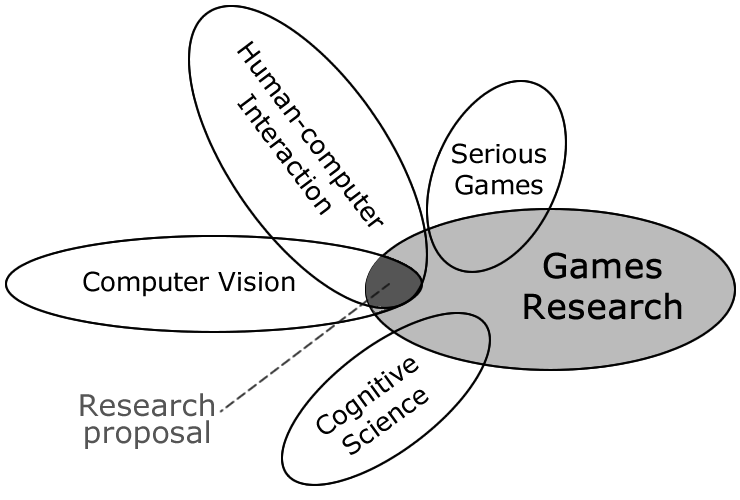
\includegraphics[scale=0.6]{Content/figures/fields}
    \caption{Different fields involved in this research. Main contribution is on the area of Games Research.}
    \label{fig:fields}
\end{figure}

The present research mainly involves and contributes to the field of games research, particularly the branch related to variations of emotions during interactions of users and games. The process of monitoring user emotions in human-computer interaction, known as affective computing \parencite{picard2000affective}, is a challenging endeavor and a recurrent research topic. This thesis brings concepts of computer vision into the field of games research to enhance the process of monitoring user emotions, making it non-obtrusive by proposing a method to remotely acquire and analyze player's signals in order to detect stress and boredom levels. As detailed in Chapter \ref{ch:literature-games} (on page \pageref{ch:literature-games}), many different theories can be used to model emotions and consequentially define stress and boredom in different contexts, including games, for instance. Despite being connected to the topic of human emotions, this research does not focus on Psychology or Cognitive Science, whose definition of stress and boredom might carry a different meaning and correlation with games. In the context of this research, the definition of emotions is less related to Psychology or Cognitive Science, instead it is based on Biology with focus on a quantitative analysis of the human physiology. The research presented in this thesis heavily relies on the fact that physiological arousal is connected to emotion regulation \parencite{appelhans2006heart,schubert2009effects}, in particular the interactions of the Autonomic Nervous System (ANS). The systems that compose the ANS interact to produce variations in the physiological signals to keep a lower or higher degree of physiological arousal, e.g. reacting to a threatening situation triggers the body to alertness, which is commonly referred to as ``fight or flight" response. As a result, both stress and boredom are defined in the scope of this thesis as emotional states that are manifestations of psychophysiological signals in the body caused by such interactions of the ANS. It is out of the scope of this thesis to create a (new) definition of stress and boredom based on the analysis of psychophysiological signals. On the contrary, the aim is to identify those emotional states based on the analysis of the previously mentioned signals and their variations. Those signals are the source of information used to classify the emotional state of subjects.

%Stress and boredom, in the context of this research, are emotions used in the games research field to describe the state of mind of players during the interaction with games. Stress, in the scope of this research, is a state of mind self-reported by a player during a game session that expresses a high level of anxiety, particularly when the player's skill level is not sufficient to beat the current challenge in the game. Similarly, boredom is a state of mind self-reported by a player during a game session that expresses a low level of enjoyment, particularly when the player's skill level is higher than the required to beat the current challenge in the game.
